\section{The genetic algorithm}
%******************************************************
\subsection{Description of genetic algorithms}
Genetic algorithms, or GA's, are based on the idea of evolution, that the most suited individuals tend to live longer and reproduce. A population is simulated in an artificial world using a combination of reproduction, gene crossover and mutation, with a given goal to achieve. The population consists of individuals, each representing a \emph{feasible  solution}. Each individual contains two forms of a solution, ``the \textit{chromosome}, which is the raw 'genetic' information (\textit{genotype}) that the GA deals with, and the \textit{phenotype} which is the expression of the chromosome in the terms of the model...''\cite{GAHandbook1}. % p. 34, Section 1.6
A chromosome contains one or more genes, which is a ``representation of a single factor value for a control factor''\cite{GAHandbook1}. %p. 34, Section 1.6
During each generation in a GA reproduction is performed to create new individuals, called children.\\\\
%% Simulate / evaluate
Due to the need to simulate the population and evaluate individuals, often multiple times, GA's are not well suited for all kind of problems. When there exists an analytical solution it may be better to use that. %% Because of?
If however the problem can be simulated both problems without analytical solutions and problem with complicated analytical solution can be handled by GA's.\\\\
%% Variations / Generational / Steady-state
There are different ways to implement genetic algorithms, with variations in how each step is performed. This yields many different versions of genetic algorithms. First there are two different kinds of GA's, steady-state and generational. Steady-state maintains and alters one population by replacing its individuals through reproduction, while generational replaces an old population with a new one. In Figure~\ref{GeneticFlowChart-generic} a flowchart of a genetic algorithm is shown. Descriptions of each step follows below.\\\\
%% Initial population
The first step is to obtain an initial population, either by an existing set of solutions or by creation.\\\\
%% Evaluation / Fitness function
To be able to compare individuals, and later determine if the goal is achieved, the individuals had to be evaluated. For that purpose a fitness function is used, which is to calculate a score for an individual depending on how well it fulfils the given goal.\label{fitnessf}
\begin{figure}[!htb]
	\centering
	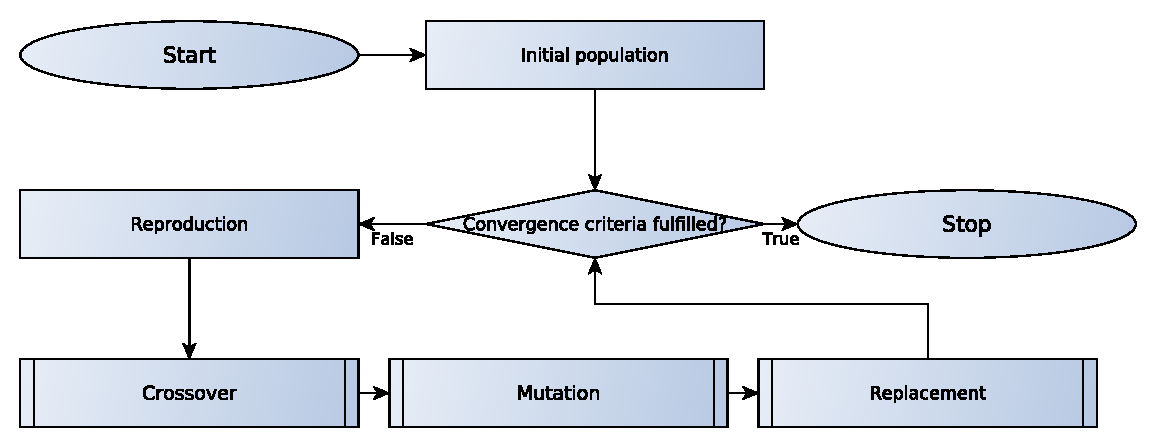
\includegraphics[width=\textwidth]{chapter_4_methods/GeneticFlowChart-Generic}
  	\caption[Flowchart of a genetic algorithm]
  	{Flowchart of a genetic algorithm.}
	\label{GeneticFlowChart-generic}
\end{figure}
%% Reproduction
\\To make the solutions evolve a reproduction step is performed, in which existing individuals in the population are combined. During this step two individuals are selected and used to create two new individuals. The new individuals are created first by crossover, in which genes are combined from the parents, and then the individual is subject to mutation. The step is thereafter repeated for the population until a desired population size is obtained.\\\\
%% Selection (parents)
There are different methods to select individuals for reproduction, of which five are Fitness Proportionate Selection, Random Selection, Fit-Fit, Tournament selection and Elite selection.
\begin{itemize}
\item In Fitness Proportionate Selection, the probability of choosing a more fit individual is higher than to select a less fit individual. One often used method is Roulette Selection.%More info?
\item In Random Selection, the probability to be selected is equal for all individuals. 
\item With Fit-Fit, at each step the two most fit individuals are selected, but the same individual can not be chosen more than once at each selection procedure.
\item Tournament selection chooses a number of individuals stochastically, and then take the best of them.
\item In Elite selection the best individual is chosen. This selection procedure should be used in combination with another selection method.
\end{itemize}
%% Crossover
For Crossover there are also different methods, such as n-point crossover and uniform crossover.
\begin{itemize}
\item In n-point crossover, the parent's chromosomes are cut into n+1 fragments from which the children receives chromosomes. The n stands for the number of fragments to be created, and the child receives chromosomes alternating between the parents, so that the first child gets the first fragment from the first parent, the second segment from the second parent, the third segment from the first parent and so on. The second child gets the first fragment from the second parent, the second fragment from the first parent, and so on.
\item In uniform crossover, ``Given two parent chromosomes of length 1, each parent copies 1/2 genes to each child, with the selection of the genes being chosen independently.''\cite{GAHandbook1}.
\end{itemize}
%% Mutation
Mutation is important in GA's since it makes sure that solutions that are not possible to find by combining individuals in the initial population can be found. It corresponds to the variance in nature when genes are copied.\\\\ % Ref
%% Replacement
When reproduction has been completed, in order to not increase the population size, a replacement is performed. For this there are several methods, such as Weak Parent, Both Parents, Weakest Individual and Random replacement.
\begin{itemize}
\item In Weak Parent, a weaker parent is replaced by a stronger child.
\item In Both Parents, the children replaces the parents.
\item In Weakest Individual, the children replaces the two weakest individuals in the population, if the children are more fit.
\item In Random replacement, the children replaces random individuals in the population.
\end{itemize}
%% Termination
To make sure the algorithm ends at some point, a termination condition has to be used, for instance a maximum number of generations, a limit in fitness sum, a median fitness, best individual or worst individual.
\begin{itemize}
\item With Fitness sum, the algorithm will terminate when the sum of the fitness for the population is less than or equal to a specified value.
\item With Median fitness, a range for the fitness is specified.
\item With best individual, the algorithm will terminate when the minimum fitness drops below a convergence value. This guarantees at least one good solution and decreases the runtime for the algorithm since the entire population does not have to converge to a solution.
\item Worst Individual is close to best individual, but as the name suggests the fitness of the worst individual is  considered instead of the best.
\end{itemize}
%% Encoding
To adapt genes to computers, an encoding has to be used.  According to literature \cite{GAHandbook1} binary encoding is the fastest encoding, where each gene is encoded as 0 and 1, but integer encoding and string encoding can also be used. If binary encoding is used, 'bit-flip' can be used for mutation, where a 0 in a gene representation is switched to a 1, or vice versa.
%******************************************************
\subsection{Development process of the genetic algorithm}\label{geneticdevelopment}
The first idea for development was to use an existing framework for Genetic Algorithms, such as LibGA \cite{libGA} %p. 146, Section 6.4.
or GAUL\cite{GAUL}, to save time on programming. Due to the implementation of the libraries, for this application it was determined to be faster to write a new implementation.\\\\
%
After reading relevant parts of the source code from existing libraries and source code that was obtained after contacting Johan Thunberg et. al., for ideas, a first attempt to a program was written. The first version was a boolean control network, where feasible solutions were generated by using a random function to generate numbers, representing moves, between 0 and 4 to indicate if the pursuer were to move left, right, up, down or stand still. For each pursuer, an integer based encoding was used, which was easy to implement and debug compared to binary encoding. An encoding based on pointers to the node in the node network (see Section 3.2) was also evaluated, but no obvious advantages were found. The algorithm was extended to a generational GA instead of steady-state, because of easier implementation and a more intuitive termination condition in number of generations.\\\\
%% Fitness
At first a simple fitness function with two variables was used, Equation \eqref{fitness1}, in which S4 is the number of \emph{tiles} in state 4 and \textit{steps} is the total number of steps taken to minimize S4.
%
\begin{equation}\label{fitness1} (1+S4+steps) \end{equation}
%
A change of selection procedure to Fitness Proportionate Selection made it necessary to switch to a function which was to be maximized, Equation \eqref{fitness2}, where the numerator was used to scale the fitness value closer to positive integer values.
%
\begin{equation}\label{fitness2} \frac{1000}{(1+S4+steps)} \end{equation}
%
The final version of the fitness function was similar to Equation \eqref{fitness2}. By using the total number of tiles, and the maximum allowed steps, called MaxSteps, the fitness function was limited to positive integer values, which should be easier for a computer to calculate, compared to the decimal values in Equation\eqref{fitness2}.
%
\begin{equation} \label{fitness3}Tiles-S4+MaxSteps-Steps \end{equation}
%
In comparison Equation \eqref{fitness2} gives a more fit individual a higher fitness value than Equation \eqref{fitness3}, but using Equation \eqref{fitness3} was not considered to be a limitation, as a high selection pressure can lead to premature convergence \cite{GAHandbook1}.\\\\
%% Selection
For selection, Random, Tournament  and Fitness Proportionate Selection were considered, all three in combination with Elite Selection. Random selection was considered the easiest to implement and was used to create a first working version of a GA, but it was replaced with Tournament selection as it gives a more fit individual an advantage. In the final version a Fitness Proportionate Selection was used, which gives more fit solutions an even greater advantage and thereby helps the population converge even faster. Elite Selection was used to make sure the two best solutions were not lost between generations.\\\\
%% Crossover
To make the crossover operation easy to implement, a version of n-point crossover was used. One path from each pursuer was used alternating from each parent.\\\\
%% Mutation
Due to the integer encoding, and node network representation, mutation by 'bit-flip' was not easily implemented. Instead a gene was selected by a random function, and thereafter a random point of the gene is chosen to be replaced. To make sure the partly modified gene corresponds to a feasible path in the environment the gene is altered from the selected part of the gene until the end of the gene.\\\\
%% Replacement
To make sure the overall fitness of the population increased, a weak parent replacement was used.\\\\
%% Parameters
At first a population size of 400 was used, which was what worked best after 10 trial runs at environments of size 5x5, in combination with a limit of 100 generations and 200 allowed steps per pursuer. Mutation frequency was set to 5\% after testing different values, which is more than the often used value in literature \cite{GAHandbook2} of 1-2\%, but still not very large. The parameters varied, and due to the increasing computation time with increasing population size a maximum of 2000 individuals was used, after trying different times for different population sizes, in combination with a high mutation rate of 75\% and a maximum of 800 generations. This was in order to examine as many different feasible solutions as possible when working with environments larger than 5x5 tiles, without having an population size of over 4.000 which at some attempts took more than 10 minutes for a single generation. The final version of the program had a more dynamic population size and step length, see Subsection \ref{geneticourproblem}.
%******************************************************
\subsection{The genetic algorithm of our problem}\label{geneticourproblem}
The final version of the genetic algorithm had a maximum population of 2000 individuals and 600 steps\footnote{Depending on the size of the environment the maximum number of steps was set between 50 and 600.}, but during initialization the population size and step length was limited to a lower value if possible. This was done by creating an initial population of 400 individuals, evaluating each and see if any complete solution was found. If so, the maximum step length is limited to the number of steps used in the complete solution, and an additional 100 individuals were added to increase the probability of having a diversity in the population. In Figure \ref{GeneticFlowChart-algorithm} a flowchart of the implemented version of a genetic algorithm is shown, with more descriptions following.
\begin{figure}[!h]
	\centering
	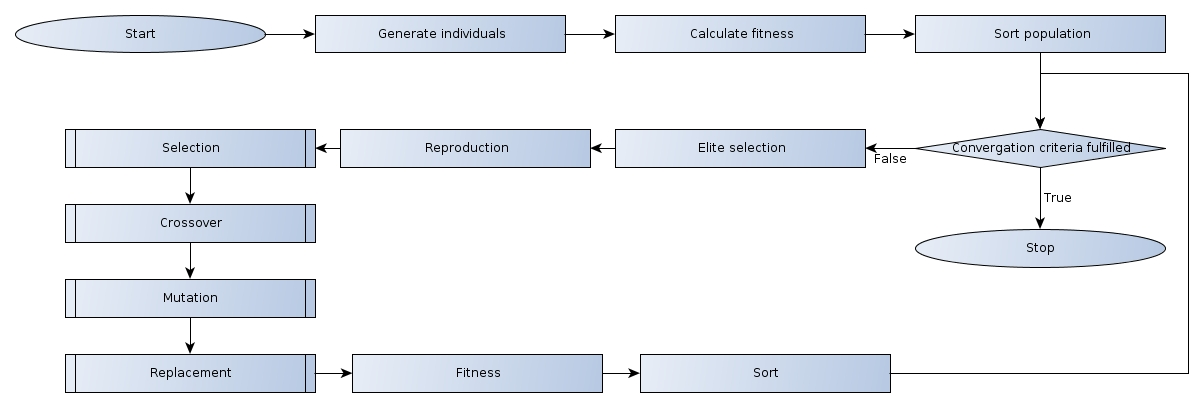
\includegraphics[width=\textwidth]{chapter_4_methods/GeneticFlowChart-Algorithm}
	\caption[Flowchart of the implemented genetic algorithm]
	{Flowchart of the implemented genetic algorithm.}
	\label{GeneticFlowChart-algorithm}
\end{figure}
%% Initial population
\\As written in Subsection \ref{geneticdevelopment} the initial population was generated by a random function, which gave each pursuer a sequence of alleles that represented each step.\\\\
%% Fitness 
Each individual was evaluated using Equation \eqref{fitness3}, and sorted by fitness in decreasing order, which facilitated selection.\\\\
%% Breeding
The two individuals with the best fitness value was added to the new population, and thereafter the selection process selected individuals for breeding. Fitness proportionate selection was used, in which a random number between 0 and the sum of the fitness of all individuals was generated. The fitness value was thereafter added for each individual, from the most to the least fit, until the number previously generated is reached, and that individual was selected. This was repeated to select a second parent. The crossover copied genes alternating between each parent, so that two different children were created. A mutation step was performed with a probability of 75\%, where a part of a gene was replaced as described in the Section \ref{geneticdevelopment}. Finally the best individuals of the parents and children were  placed in the new population, and the reproduction repeated until a new population of the same size as the previous was created.\\\\
%% Termination
As a termination criteria the fitness score of up to 99\%\footnote{Values between 50\% and 99\% was used.} of the individuals in the population was compared. If the individuals compared both were a \emph{complete solution} and had and had an equal fitness score, the algorithm was terminated. As 99\% is a very high convergence criteria, it was only used for small environments to avoid premature termination. As a second termination criteria the maximum number of generations was set to 800, to make sure the algorithm would terminate even if no solution was found.
%******************************************************
\subsection{Our implementation of the genetic algorithm}
The algorithm was implemented using ANSI C. Every time a random value was to be obtained the command:
\begin{verbatim}
((int)((double)rand() / ((double)RAND_MAX + 1)*SCALE_FACTOR))
\end{verbatim}
was called, which generates a number in the range [0,SCALE\_FACTOR). For random seed number
\begin{verbatim}
srand(time(0))
\end{verbatim}
was used. No alternative random functions were evaluated during the development.\\\\
The population was implemented as an array, which was sorted between each generation using quicksort\cite{quicksort} in descending order after fitness value. Each individual was represented by a struct containing the number of nodes in \emph{state} 4, the length of a \emph{path} needed to reach a \emph{complete solution}, a gene for each pursuer and the fitness score. Each gene represented a \emph{path} for a pursuer.\\\\
%
To avoid premature convergence to an \emph{incomplete solution}, a modification to the termination condition was made. For each individual the number of \emph{tiles} in \emph{state} 4 was kept, so that even if the population had the same fitness value the algorithm would not terminate unless a \emph{complete solution} was found.
\newpage